\begin{columns}[totalwidth=.85\linewidth]
	\column{\textwidth}
	\vspace{-10mm}

		\begin{itembox}[l]{Classical Theory of Rubber Elasticity}
			% \begin{block}{Free Energy Density of Rubbers against Strain invariant}
			% 	\vspace{-2mm}
				% 非圧縮性条件から第3不変量がおちて、
				% Free Energy Density of Rubbers against Strain Invariant
			% 	\small
			% 	\begin{align*}
			% 		\dfrac{F}{V} = W 
			% 		% &= \sum_{i,j = 0}^{\infty} C_{ij}(I_1-3)^i(I_2-3)^j \\[-2mm]
			% 		&= C_0 + \underbrace{{\color{green}C_1(I_1-3)} + {\color{red}C_2(I_2-3)}}_{\color{red}Mooney-Rivlin Model} + \sum_{i,j = 1}^{\infty} C_{ij}(I_1-3)^i(I_2-3)^j
			% 	\end{align*}  
			% % \end{block}
			% % \vspace{-5mm}
			% \begin{columns}[T, onlytextwidth]
			% 	\column{.48\linewidth}
			% 		\begin{itembox}{Neo-Hookean Model}
			% 			% \vspace{-2mm}
			% 			% 第1不変量のみを対象
			% 				\small
			% 				\begin{align*}
			% 					&W = C_1 (I_1-3) \\
			% 					&\text{against Uniaxial elongation} \\
			% 					&\sigma_{nom} = 2 C_1\left(\lambda - \dfrac{1}{\lambda^2}\right) = G \left(\lambda - \dfrac{1}{\lambda^2}\right)
			% 				\end{align*}
			% 		\end{itembox}
			% 	\column{.48\linewidth}
			% 		\begin{itembox}{Mooney-Rivlin Model}
			% 			% \vspace{-2mm}
			% 			% 高次の項をおとす
			% 			\small
			% 			\begin{align*}
			% 				&W = C_1 (I_1-3) + C_2(I_2-3) \\
			% 				&\text{against Uniaxial elongation} \\
			% 				&\sigma_{nom} = 2 \left(C_1 + C_2\dfrac{1}{\lambda} \right) \left(\lambda - \dfrac{1}{\lambda^2}\right)
			% 			\end{align*}
			% 		\end{itembox}
			% \end{columns}
			% \vspace{-1mm}
			\begin{itembox}{With or without Junction Poinits fluctuation}
				\vspace{5mm}
				\begin{columns}[T, onlytextwidth]
					\column{.45\linewidth}
					\vspace{5mm}
					% \small
					\color{blue}{Affine Network Model\cite{flory1}
					}
					\vspace{2mm}
					% \small
					\begin{align*}
						% &\text{Affine Network Model}\\
						&G_{affine} = \nu k_B T  \\
						&\text{$\nu$: Number density of strands}
					\end{align*}
					\column{.45\linewidth}
					\vspace{5mm}
					% \small
					\color{red}{Phantom Network Model\cite{james}
					}
					\vspace{2mm}
					% \small
					\begin{align*}
						% &\text{Phantom Network Model}\\
						&G_{phantom} = \nu k_B T \left(1 - \dfrac{2}{f}\right) \\
						&\text{$f$: Functionality of Junction Points}
					\end{align*}
					\normalsize
				\end{columns}
			\end{itembox}
		\end{itembox}


	\begin{itembox}[l]{Recent approach for Constraints (Entanglements)}
		\begin{itemize}
			\item Diffused-Constraint Model\cite{erman}
			\begin{itemize}
				\normalsize
				\item Confining potential affect all points along the chain.
				% \footnote{\tiny{A. Kloczkowski, J.E. Mark, B. Erman, Macromol., 28, 5089 (1995)}}
			\end{itemize}
			\item Nonaffine Tube Model\cite{Rubinstein1}
			\begin{itemize}
				\normalsize
				\item Improved model of "Edwards' Tube Model".
				% \footnote{\tiny{M. Rubinstein, S. Panyukov, Macromol., 30, 25, 8036 (1997)}}
			\end{itemize}
			\item Slip-tube Model\cite{Rubinstein2}
			\begin{itemize}
				\normalsize
				\item A pairwise interaction of chains is introduced.
				% \footnote{\tiny{M. Rubinstein, S. Panyukov, Macromol., 35, 6670 (2002)}}
			\end{itemize}
		\end{itemize}
	
		\begin{columns}[totalwidth=1\textwidth]
			\column{.65\textwidth}
			% \small
			\begin{align*}
				&f^*(\lambda^{-1}) = G_c + \dfrac{G_e}{0.74 \lambda + 0.61 \lambda^{-1/2} - 0.35} \\
				&G_c = \nu k_B T \left(1-\dfrac{2}{\phi} \right), \quad G_e = \dfrac{4}{7} \nu k_B T L \\
				% &\text{where $\nu$ is the number density of network chains,} \\
				& \text{L is the number of slip-links per network chain}
			\end{align*}
			\column{.3\textwidth}
			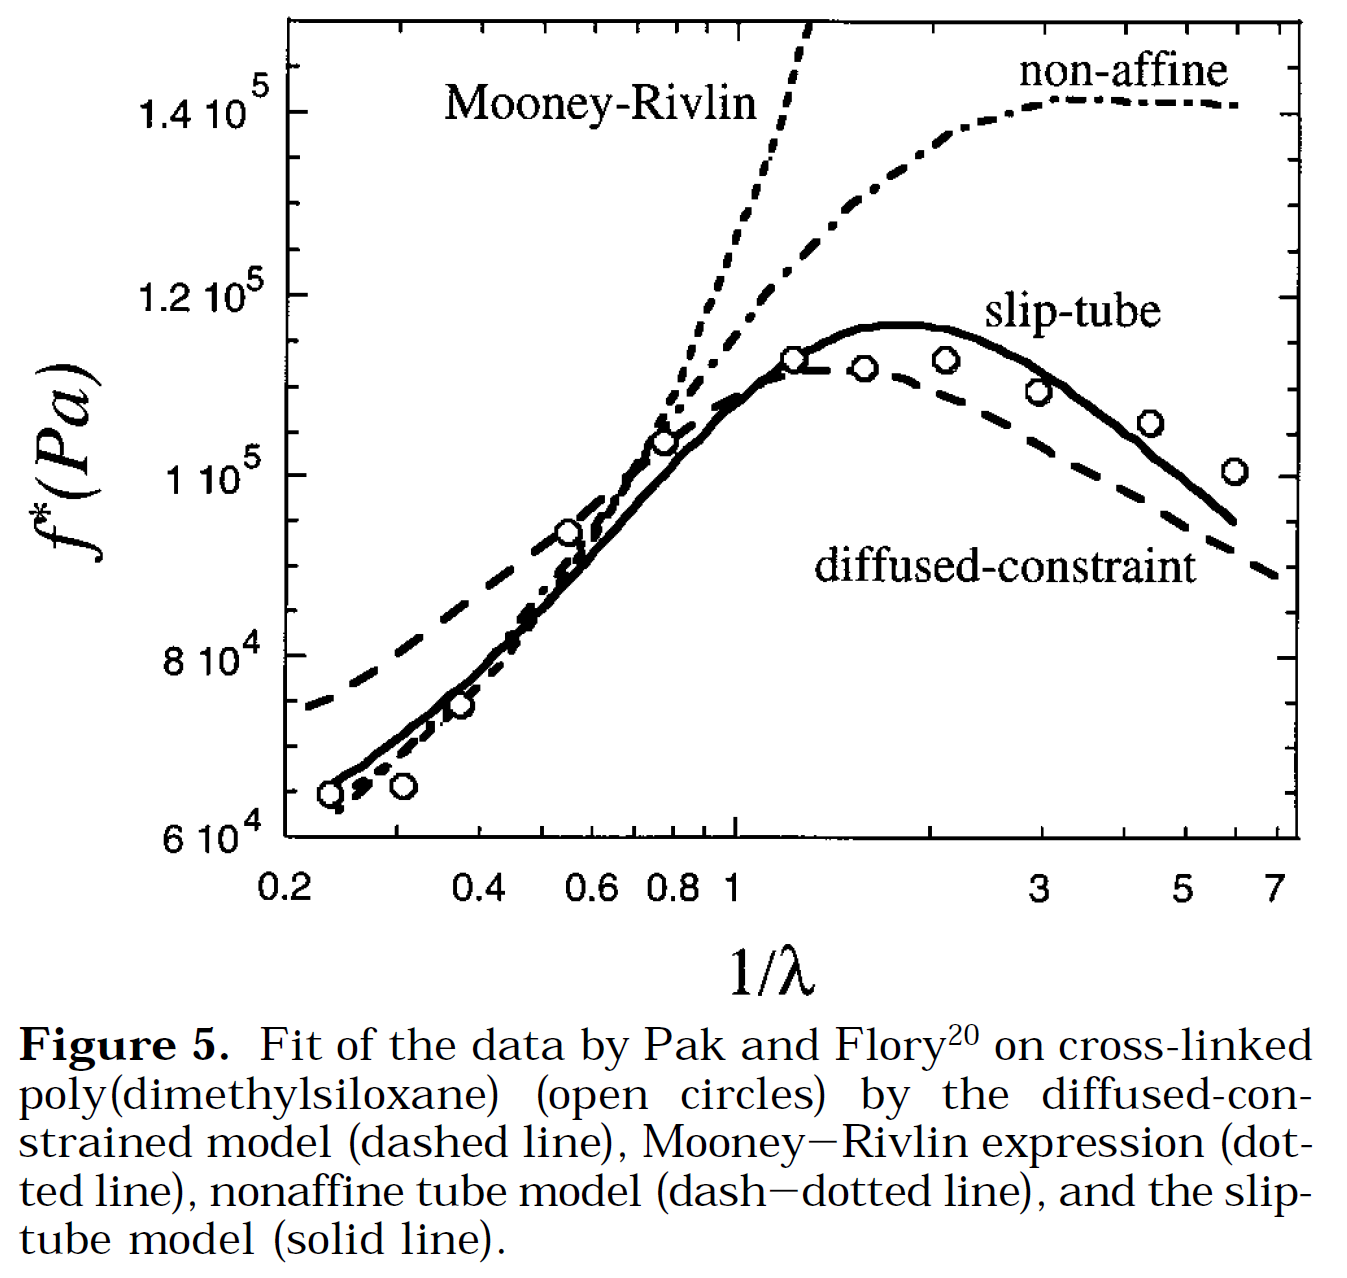
\includegraphics[width=\textwidth]{NW_model_rubinstein.png}
		\end{columns}
	\end{itembox}

	\begin{itembox}[l]{Random Connectivity\cite{flory2}}
		\begin{columns}[totalwidth=\textwidth]
			\column{.65\textwidth}
				\begin{itemize}
					\item Regular Structure as Initial Structure
					\begin{itemize}
						\normalsize
						\item Same strand length for easy understanding
						\item Easy to monitor the strand length distributions
					\end{itemize}
					\item Irregular Connectivity for each Junction Point
						\begin{itemize}
							\normalsize
							\item Random Connectivity
							\item Fluctuations of Junction Points are secured
						\end{itemize}
					\item Phantom Network Requirement by Flory is fulfilled
				\end{itemize}
			\column{.3\textwidth}
				\centering
				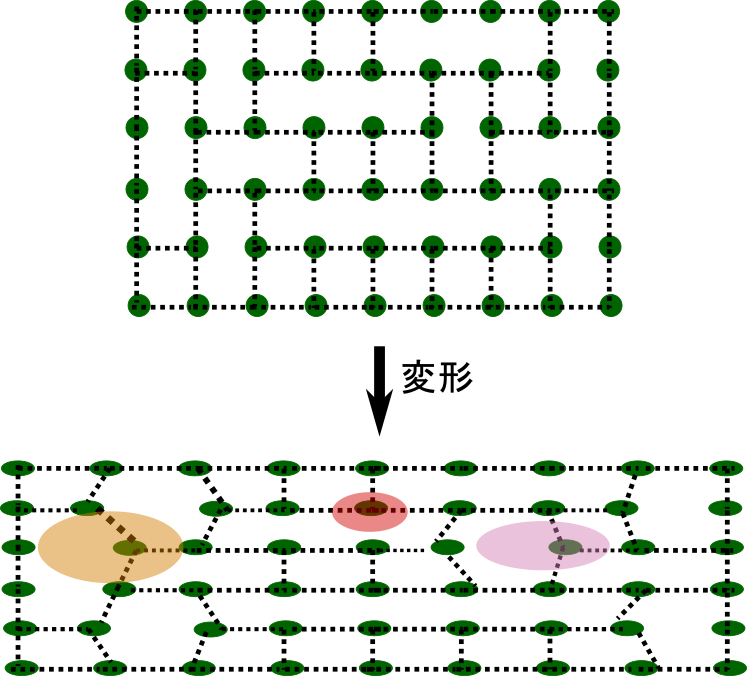
\includegraphics[width=\textwidth]{random_NW.png}
		\end{columns}
	\end{itembox}

	\begin{itembox}[l]{OBJECTIVE}
		\begin{itemize}
			\item Recent approach for rubber elasticity models are based on Phantom Network Model.
			\item To investigate the criteria for Phantom Network Model, employing phantom chain 
			as strand and introducing random connectivity, MD simulation studies were carried out.
        \end{itemize}
	\end{itembox}
\end{columns}